% !TEX root = ../main.tex

\section{Introduction}
In this report, we attempt to validate the experimental results of ``BBR:
Congestion-based Congestion Control''~\cite{cardwell2016bbr}. We start
by looking at the goals, motivations and results from the BBR
\cite{cardwell2016bbr} paper.

\para{Goals}
What was the original paper trying to solve?

The original paper was trying to find a congestion control approach
that would stay as close as possible to optimal network operating point
in various network conditions. The network link is operating at the optimal
point when bandwidth utilization is maximized and latency is minimized.

\para{Motivation}
Why is the problem important/interesting?

This is importannt problem to tackle because traditional congestion control
algorithms such as CUBIC have a tough time operating efficiently when there
is non-negligible packet loss on the packet. This limitation comes from the
CUBIC's use of packet loss as a signal for congestion, which can unnecesarily
hinder throughput leading to poor performance.


\para{Results}
What did the original authors find?

The BBR paper descibes a new form of congestion control that is based on actual
congestion going in the network. The insight from the authors is that their
approach estimates bottleneck bandwidth and then bottleneck latency in succession
so as to be able to get as close as possible to the ideal operating point of
maximum bandwidth and minimal latency.

The core finding is that BBR outperforms CUBIC for loss rates above 0.1\%. Here's
the a graph showing the performance comparison between BBR and CUBIC.


\begin{figure}[h]
  \centering
  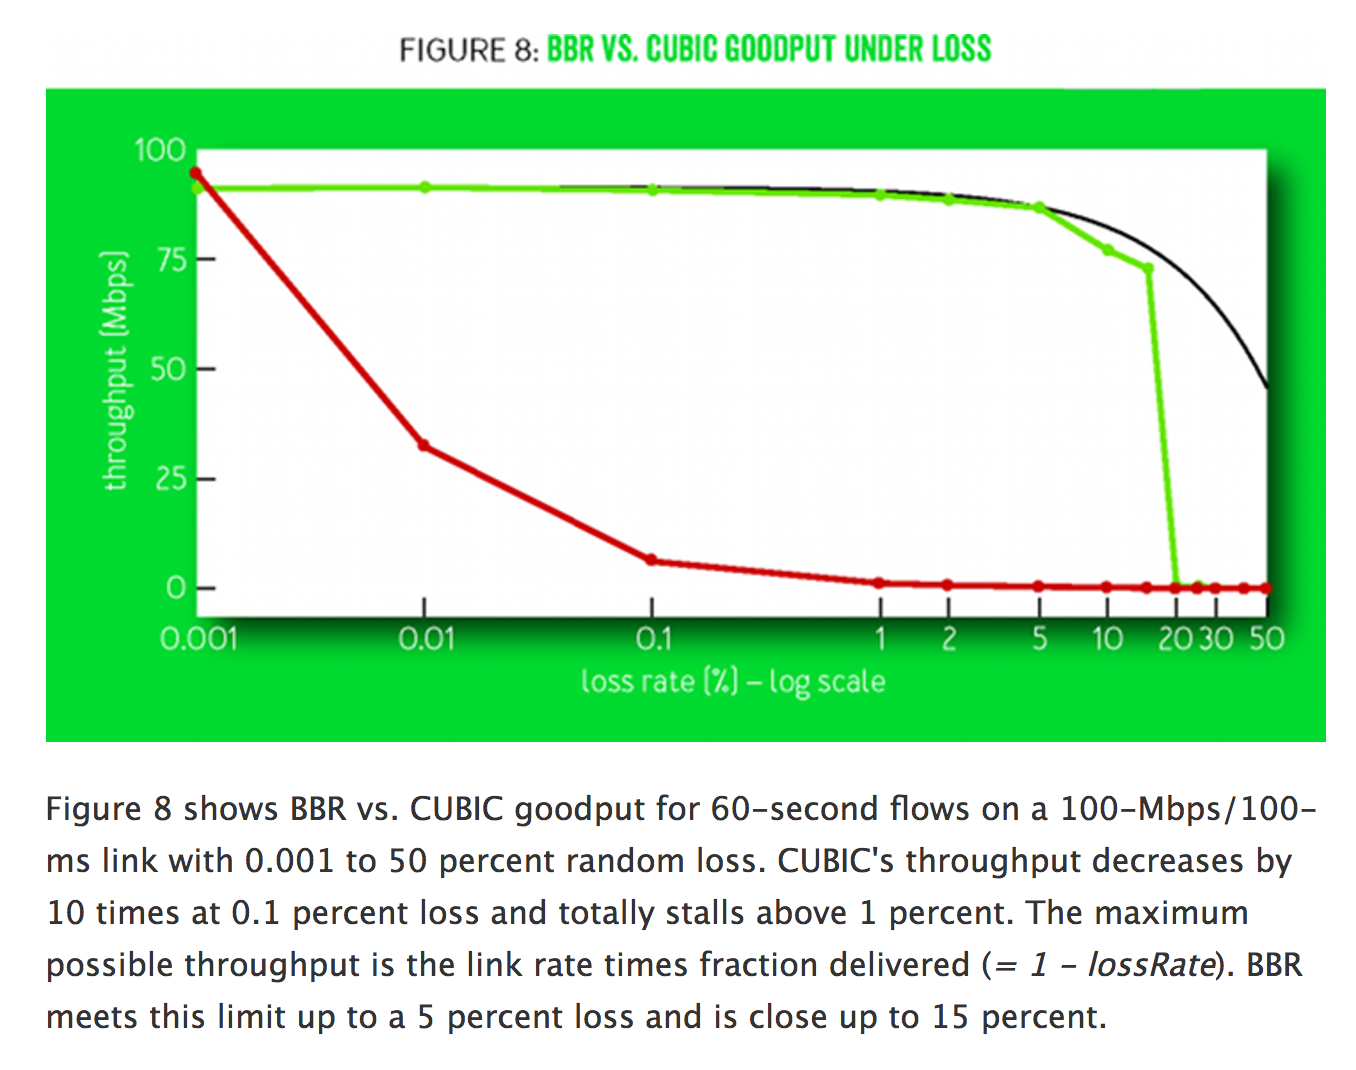
\includegraphics[height=3cm]{./img/bbr_fig8.png}
  \caption{Throughput vs 95-percentile Signal Delay for simple AIMD.}
  \label{fig:exb}
\end{figure}